\documentclass[12pt,a4paper]{article}
\usepackage[T1]{fontenc}
\usepackage{multicol}
\usepackage{booktabs}
\usepackage{graphicx}

\graphicspath{ {./img/} }
\title{Raport z monitorowania ruchu sieciowego}
\author{Radosław Wojtczak, Michał Krosny\\ 254607,256791}

\begin{document}
    \maketitle
    \newpage
    \section{Przeprowadzone badania ruchu sieciowego} 
        \begin{center}
            \begin{tabular}{|c|c|}
                \hline
                Lokalizacja & Nazwa AP\\
                \hline
                Lubin Cuprum Arena & Free WiFI\\
                Wrocław Wroclavia & Wroclavia Free\\
                Wrocław Wroclavia & Free wifi\\
                Wrocław Wroclavia & Open WiFi\\
                Wrocław Dworzec Gł. & Open WiFi\\
                KD Wrocław-Lubin & Open Free WiFi\\
                \hline
            \end{tabular}
        \end{center}~\\
        Zgodnie z poleceniem zadania karta sieciowa laptopa została ustawiona w tryb monitorowania \textit{promiscuous mode}. Następnie zostały udostępnione sieci Wi-Fi o różnych nazwach, w różnych lokalizacjach, co prezentuje powyższa tabela. Otrzymane dane zostały zebrane przy pomocy programu WireShark. \\
        Badania trwały od 20 do 50 minut i tylko dwa z nich zakończyły się zaobserwowaniem jakiegokolwiek ruchu.
        Były to ap: Wroclawia pod nazwą Free WiFi oraz KD Wrocław-Lubin pod nazwą Open Free WiFi.
    
    
    \section{Wyszukiwane SSID}
        Czytanie danych odbywało się poprzez sprawdzanie pakietów, gdzie typ był równy "probe request". 
        Wartości nazywane jako "wildcard" w tym sprawozdaniu zosały pominięte.
        Badanie przeprowadzone w lokalizacji Cuprum Arena Lubin:\\
        \begin{small}
            \begin{multicols}{3}
                3792\\Stage\\emil\\l\\P20Pro\\EDV\\EDV\_5G\\McD-Hotspot\\UPC39A47D5\\B593-8457\\AndroidAP\\
                potaczek\\eBos\\UPC242544703\\sala19.local\\Tofik97\\DWR-932\_DDEC06\\
                Livebox-BC16\\DWR-116\_C42C12\\willa3\\PARK\_ROZRYWKI\\NETIASPOT-2.4GHz-4de5\\NETIASPOT-E58B60\\
                ING Internet\\UPC4850294\\Lenovo TAB4 10\\Klient\\wksraclawicka\\DWR-960\_83236D\\HUAWEI-B535-03D8\\
                NETIASPOT-866470\\NETIASPOT-2.4GHz-awwT\\CircleHostel\\NETIASPOT-BA0E70\\iphone mateusx\\
                netiaspot-ds44co\\PizzaHut Hotspot\\Cuprum-Arena-A\\RESTAURACJA\\UPC244749285\\zosiaaa\\SUSHIdlaMNIE\\
                HUAWEI-14B7\\ARKA\_D\\CPE\_B8EDB9\\UPC9939797\\COSTA COFFEE\\0028635B\\null\\HUAWEI-E5186-2FF4\\
                MikroTik-6187F0\\EuroWeek123\\UPCC6A6EA2\\PHILIPS\\MikroTik-6187F1\\TP-LINK\_ECCAD2\\
                ROBOT\#\#\#c3-aa-f7\\Osiek2\\orange\\marzec\\Redmi\\seaside\\tmobile\\AndroidAP12\\Internet\_Domowy\_4A302F\\
            \end{multicols}
        \end{small}

    \section{Podłączeni użytkownicy}
        \begin{center}
            \begin{tabular}{|c|c|}
                \hline
                Free WiFi & Open Free WiFi\\
                \hline
                06:b1:34:3f:97:e0 & 30:45:96:1b:e9:ba\\
                f2:56:d9:85:67:1f & 88:11:96:83:46:b1\\
                \hline
            \end{tabular}
        \end{center}
        Przy pomocy zakładki "Statystyka" w programie WireShark została sporządzona powyżsża lista unikalnych adresów MAC podłączony do sieci. \\
        Pozostałe badania zakończyły się zerową ilością połączeń. \\
        Ograniczona liczba użytkowników znacząco wpłynęła na ograniczoną liczbę danych otrzymanych w ramach eksperymentu. Zauważamy, że jedyni użytkownicy zalogowali się, gdy nazwa sieci posiadała w sobie frazy "Free", "WiFi" czy "Open".

    \section{Odwiedzane strony}
        Dokonując analizy odwiedzanych stron przez użytkowników zauważamy, że
            \begin{itemize}
                \item Użytkownicy mimo korzystania z otwartej sieci wciąż łączą się z takimi stronami jak \textit{www.google.com, www.linkedin.com}, czy \textit{www.wp.pl}
                \item Część z otrzymanych serwisów (Przykład: \textit{connectivitycheck.android.com}) są serwisami, których zadaniem jest sprawdzenie, czy urządzenie wciąż jest połączone z internetem.
            \end{itemize}
        \textbf{KD Lubin-Wrocław:}\\
        \begin{scriptsize}
            \begin{multicols}{3}
                \begin{center}
                        adservice.google.com\\android.clients.google.com\\android.googleapis.com\\
                        api.gameanalytics.com\\app-measurement.com\\b-graph.facebook.com\\cdn.ampproject.org\\
                        cdn.playa-games.com\\cfg.sfgame.de\\chat-e2ee-mini.facebook.com\\clients3.google.com\\
                        connectivitycheck.android.com\\connectivitycheck.gstatic.com\\content-autofill.googleapis.com\\
                        dimg-pa.googleapis.com\\edge-mqtt.facebook.com\\encrypted-tbn0.gstatic.com\\
                        encrypted-tbn1.gstatic.com\\encrypted-tbn2.gstatic.com\\encrypted-tbn3.gstatic.com\\g.whatsapp.net\\
                        geller-pa.googleapis.com\\googleads.g.doubleclick.net\\graph.facebook.com\\growth-pa.googleapis.com\\
                        i.ytimg.com\\inbox.google.com\\infinitedata-pa.googleapis.com\\launches.appsflyer.com\\
                        lh3.googleusercontent.com\\lh5.googleusercontent.com\\lookaside.facebook.com\\mail.google.com\\
                        mtalk.google.com\\notifications-pa.googleapis.com\\peoplestack-pa.googleapis.com\\play.googleapis.com\\
                        play-fe.googleapis.com\\play-lh.googleusercontent.com\\scontent.ftxl2-1.fna.fbcdn.net\\ssl.gstatic.com\\
                        static.whatsapp.net\\store.hispace.hicloud.com\\time.android.com\\video.fpoz6-1.fna.fbcdn.net\\
                        w51.sfgame.net\\www.google.com\\www.googleadservices.com\\www.googleapis.com\\www.gstatic.com\\
                        xtrapath2.izatcloud.net\\youtubei.googleapis.com\\
                \end{center}
            \end{multicols}
        \end{scriptsize}

        \textbf{Wroclavia:}\\
        \begin{scriptsize}
            \begin{multicols}{3}
                \begin{center}
                    11603.lsapp.eu\\26-courier.push.apple.com\\34-courier.push.apple.com\\3pd.am5.vip.prod.criteo.com\\
                    3pd.criteo.com\\safeframe.googlesyndication.com\\a.teads.tv\\
                    a1744.dscg2.akamai.net\\a1813.dscd.akamai.net\\a1845.dscg2.akamai.net\\a1931.dscgi3.akamai.net\\
                    a1958.dscd.akamai.net\\a2047.dscb.akamai.net\\aax-eu.amazon-adsystem.com\\abs-0.twimg.com\\abs-zero.twimg.com\\
                    ad.doubleclick.net\\ads.businessclick.com\\ads.mopub.com\\adservice.google.com\\adservice.google.pl\\
                    adx.adform.net\\ams01.search.spotxchange.com\\api.flightproxy.teams.microsoft.com\\api2.branch.io\\
                    api3.cc.skype.com\\api-glb-euc1a.smoot.apple.com\\cloudapp.net\\
                    api-v3.tinypass.com\\app.snapchat.com\\app-analytics-v2.snapchat.com\\apple.com\\app-measurement.com\\
                    apresolve.spotify.com\\assets-jpcust.jwpsrv.com\\
                    authorisation.grupaonet.pl\\authsvc.teams.microsoft.com\\aws.api.sc-gw.com\\aws.api.snapchat.com\\
                    aws.duplex.snapchat.com\\axel-springer-pl-d.openx.net\\b101.s372.meetrics.net\\bc.wp.pl\\
                    bidder.am5.vip.prod.criteo.com\\bidder.criteo.com\\bidder.par.vip.prod.criteo.com\\
                    blob.byaprdstr10a.store.core.windows.net\\bolt-gcdn.sc-cdn.net\\buy.tinypass.com\\c.amazon-adsystem.com\\
                    c2.piano.io\\safeframe.googlesyndication.com\\captive.apple.com\\
                    captive.g.aaplimg.com\\cb.mopub.com\\safeframe.googlesyndication.com\\
                    cc-euwe-05-skype.cloudapp.net\\cdn.apple-mapkit.com\\cdn.branch.io\\cdn.brandmetrics.com\\cdn.jwplayer.com\\
                    cdn.syndication.twimg.com\\cdn.tinypass.com\\cf-st.sc-cdn.net\\chat-e2ee-mini.c10r.facebook.com\\
                    chat-e2ee-mini.facebook.com\\chatsvcagg.teams.microsoft.com\\cl2.apple.com\\cl5.apple.com\\
                    clients.config.office.net\\clients.l.google.com\\clients1.google.com\\clients3.google.com\\cmp.dreamlab.pl\\
                    codepush.blob.core.windows.net\\codepush.teams.microsoft.com\\collector.brandmetrics.com\\
                    config.teams.microsoft.com\\config-chr.health.apple.com\\configuration.ls.apple.com\\connect.facebook.net\\
                    contentsync.onenote.com\\cosmic-eastus-ns-8f4565d3f227.trafficmanager.net\\cs386.wpc.edgecastcdn.net\\
                    cs45.wac.edgecastcdn.net\\cs491.wac.edgecastcdn.net\\csi.gstatic.com\\csr.onet.pl\\d1v810m8ywaj43.cloudfront.net\\
                    d1ykf07e75w7ss.cloudfront.net\\d2iv48hg4yxj1k.cloudfront.net\\dart.l.doubleclick.net\\dealer.spotify.com\\
                    delivery.clickonometrics.pl\\df.trap.teams.microsoft.com\\dual-spo-0004.spo-msedge.net\\e10499.dsce9.akamaiedge.net\\
                    e11290.dspg.akamaiedge.net\\e1329.g.akamaiedge.net\\e14868.dsce9.akamaiedge.net\\e3811.e9.akamaiedge.net\\
                    e4466.g.akamaiedge.net\\e6987.dsce9.akamaiedge.net\\e69896.dscapi6.akamaiedge.net\\e8037.i.akamaiedge.net\\
                    e9957.b.akamaiedge.net\\edge-mqtt.facebook.com\\edge-web.dual-gslb.spotify.com\\eduwroclaw.sharepoint.com\\
                    eduwroclaw-my.sharepoint.com\\embed.dugout.com\\emea.ng.msg.teams.microsoft.com\\entitlements.jwplayer.com\\
                    eqx.smartadserver.com\\etoto-platform.onet.pl\\euaz.tr.teams.microsoft.com\\eu-central-courier-4.push-apple.com.akadns.net\\
                    eudb.clients.config.office.akadns.net\\europe-west1-gcp.api.snapchat.com\\eu-west1-aws.duplex.sc-gw.com\\
                    events.ocdn.eu\\experience.tinypass.com\\external.fpoz6-1.fna.fbcdn.net\\external.xx.fbcdn.net\\facebook.com\\
                    fastlane.rubiconproject.com\\fbcdn.net\\fbs.smoot.apple.com\\fbsbx.com\\firebaselogging-pa.googleapis.com\\
                    flightproxy-ukso-02-teams.cloudapp.net\\fonts.googleapis.com\\fonts.gstatic.com\\fonts.wpcdn.pl\\gapl.hit.gemius.pl\\
                    gateway.facebook.com\\gateway.fe.apple-dns.net\\gateway.icloud.com\\gcp.api.sc-gw.com\\gcp.api.snapchat.com\\
                    gcs.sc-cdn.net\\gde-default.hit.gemius.pl\\get-bx.g.aaplimg.com\\go.microsoft.com\\go.trouter.teams.microsoft.com\\
                    googleads.g.doubleclick.net\\googleads4.g.doubleclick.net\\google-analytics.com\\graph.facebook.com\\graph.instagram.com\\
                    grid.bidswitch.net\\gs-loc.apple.com\\gs-loc.ls-apple.com.akadns.net\\gsp10-ssl.apple.com\\gsp10-ssl.ls-apple.com.akadns.net\\
                    gsp64-ssl.ls.apple.com\\gsp64-ssl.ls-apple.com.akadns.net\\gsp85-ssl.ls.apple.com\\gsp85-ssl.ls2-apple.com.akadns.net\\
                    gspe12-ssl.ls.apple.com\\gspe19-ssl.ls.apple.com\\gspe35-ssl.ls.apple.com\\gspe76-ssl.ls.apple.com\\gspe79-ssl.ls.apple.com\\
                    gsp-ssl.ls.apple.com\\gstaticadssl.l.google.com\\gtq.sct.sc-prod.net\\gum.am5.vip.prod.criteo.com\\gum.criteo.com\\
                    gum.par.vip.prod.criteo.com\\guzzoni.apple.com\\hbopenbid.pubmatic.com\\hbopenbid22000nf.pubmatic.com\\
                    hierarchyapi.onenote.com\\htlb.casalemedia.com\\https://app-measurement.com/sdk-exp\\i.connectad.io\\i.instagram.com\\
                    i.scdn.co\\ib.adnxs.com\\ib.anycast.adnxs.com\\ic3.events.data.microsoft.com\\images.bitmoji.com\\imasdk.googleapis.com\\
                    impala-external-lb-1441126057.us-east-1.elb.amazonaws.com\\inappcheck.itunes.apple.com\\inappcheck-lb.itunes-apple.com.akadns.net\\
                    instagram.c10r.instagram.com\\instagram.com\\instagram.fpoz6-1.fna.fbcdn.net\\iphone-ld.apple.com\\jwplayer-dualstack.map.fastly.net\\
                    kropka.onet.pl\\l-0005.l-msedge.net\\lb.\_dns-sd.\_udp.0.0.0.10.in-addr.arpa\\lb.\_dns-sd.\_udp.0.0.42.10.in-addr.arpa\\
                    lb.\_dns-sd.\_udp.253.27.128.10.in-addr.arpa\\lcdn-locator.apple.com\\lcdn-locator-usuqo.apple.com.akadns.net\\liveblog-push.dreamlab.pl\\
                    liveblog-talos.dreamlab.pl\\login.microsoftonline.com\\login5.spotify.com\\lookaside.facebook.com\\ls.hit.gemius.pl\\m.facebook.com\\
                    mamls-prod-weu-ip.westeurope.cloudapp.azure.com\\mamservice.manage.microsoft.com\\mask.apple-dns.net\\mask.icloud.com\\me.apple-dns.net\\
                    media-shield.jwplayer.map.fastly.net\\mesu.apple.com\\metrics.icloud.com\\mqtt.c10r.facebook.com\\ms.sc-jpl.com\\
                    msgapi-prod-weu-azsc1-1.cloudapp.net\\msgr-latest.c10r.facebook.com\\mvm.snapchat.com\\mvp.onet.pl\\naanalle.pl\\
                    netcts.cdn-apple.com\\nlb-aws-fr-verona-b3549c64d24264e3.elb.eu-central-1.amazonaws.com\\nstrp.adform.net\\ocdn.eu\\ocsp2.apple.com\\
                    onedscolprdcus12.centralus.cloudapp.azure.com\\onedscolprdeus00.eastus.cloudapp.azure.com\\onedscolprdwus11.westus.cloudapp.azure.com\\
                    onet.hit.gemius.pl\\pagead2.googlesyndication.com\\pagead46.l.doubleclick.net\\pagead-googlehosted.l.google.com\\parasol.wroclaw.pl\\
                    partnerad.l.doubleclick.net\\pbs.twimg.com\\pixel.wp.pl\\platform.twitter.com\\player-api.dreamlab.pl\\pop-esv5.mix.linkedin.com\\
                    prd.jwpltx.com\\prebid-eu.creativecdn.com\\prebid-server.rubiconproject.com\\prebid-server-perf-eu.rubiconproject.net.akadns.net\\
                    presence.teams.microsoft.com\\prg.smartadserver.com\\pro-accounts.snapchat.com\\profiles.tagger.opecloud.com\\pulsembed.eu\\
                    px.ads.linkedin.com\\rt.inistrack.net\\rupload.facebook.com\\s.mopub.com\\s.sc-cdn.net\\s0.2mdn.net\\s-0005.s-msedge.net\\
                    s0-2mdn-net.l.google.com\\s1.adform.net\\s372.meetrics.net\\s372.mxcdn.net\\sb.scorecardresearch.com\\scdnco.spotify.map.fastly.net\\
                    scontent.fpoz6-1.fna.fbcdn.net\\scontent.xx.fbcdn.net\\scontent-frx5-1.cdninstagram.com\\search.spotxchange.com\\
                    securepubads.g.doubleclick.net\\self.events.data.microsoft.com\\setup.fe.apple-dns.net\\setup.icloud.com\\s-eu-1.pushpushgo.com\\
                    sgqcvfjvr.onet.pl\\smoot-feedback.v.aaplimg.com\\smoot-searchv2-euc1a.v.aaplimg.com\\snap.api.mapbox.com\\spclient.wg.spotify.com\\
                    sportowefakty.wp.pl\\star.c10r.facebook.com\\star-mini.c10r.facebook.com\\static.am5.vip.prod.criteo.net\\static.criteo.net\\
                    static.doubleclick.net\\static.par.vip.prod.criteo.net\\static.xx.fbcdn.net\\static-doubleclick-net.l.google.com\\
                    statics.teams.cdn.office.net\\stats.g.doubleclick.net\\stats.l.doubleclick.net\\substrate.office.com\\swallow.apple.com\\
                    swallow-apple-com.v.aaplimg.com\\SXF-efz.ms-acdc.office.com\\syndication.twitter.com\\tagged-by.rubiconproject.net.akadns.net\\
                    tagger.opecloud.com\\teams.events.data.microsoft.com\\teams.microsoft.com\\time.apple.com\\
                    tmsg-euno-azsc-01-csa-dns.northeurope.cloudapp.azure.com\\tpc.googlesyndication.com\\tr.teams.microsoft.com\\track.adform.net\\
                    track-eu.adformnet.akadns.net\\us-central1-gcp.api.snapchat.com\\us-east1-aws.api.snapchat.com\\us-east4-gcp.api.sc-gw.com\\
                    us-east4-gcp.api.snapchat.com\\v.wpimg.pl\\video.fpoz6-1.fna.fbcdn.net\\videos-fms.jwpsrv.com\\
                    waws-prod-am2-391-d5b3.westeurope.cloudapp.azure.com\\weather-data.apple.com\\weather-data.apple.com.akadns.net\\weather-edge.apple.com\\
                    weather-edge.news.apple-dns.net\\web.facebook.com\\websocket.wp.pl\\wirtualn-d.openx.net\\world-gen.g.aaplimg.com\\wp.hit.gemius.pl\\
                    wpcdn.pl\\www.apple.com\\www.facebook.com\\www.google.com\\www.google.pl\\www.google-analytics.com\\www.googletagmanager.com\\
                    www.googletagservices.com\\www.icloud.com\\www.linkedin.com\\www.microsoft.com\\www.przegladsportowy.pl\\www.spotify.com\\
                    www.tm.ak.prd.aadg.akadns.net\\www.wp.pl\\www.youtube.com\\www-google-analytics.l.google.com\\www-googletagmanager.l.google.com\\
                    youtubei.googleapis.com\\
                \end{center}
            \end{multicols}
        \end{scriptsize}
        \newpage
    \section{Wykorzystywane protokoły i usługi}
        \begin{multicols}{2}
            \begin{center}
                \textbf{Wroclavia:}\\
                Usługi na podstawie portów:\\
                http\\
                https\\
                hpvirtgrp\\
                afs3-fileserver\\~\\

                Protokoły:\\
                TCP\\
                TLSv1.2\\
                SSL\\
                ARP\\
                MDNS\\
                XID\\
                ICMPv6\\
                DHCP\\
                ICMP\\
                DNS\\
                HTTP\\
                MPTCP\\
                IGMPv2\\
                TLSv1.3\\
                SSLv2\\
                QUIC\\
                XMPP/XML\\
                NTP\\
                TLSv1\\
                
                \vfill\null
                \columnbreak

                \textbf{KD Lubin-Wrocław:}\\
                Usługi na podstawie portów:\\
                http\\
                unisys-eportal\\
                asihpi\\
                https\\
                blp5\\
                caerpc\\
                turbonote-1\\
                invision-ag\\
                robotraconteur\\
                ssr-servermgr\\
                ortec-disc\\
                f1-control\\
                qdb2service\\
                z-wave-s\\
                m3da-disc\\
                kastenxpipe\\
                crescoctrl-disc\\
                csccfirewall\\~\\
                
                Protokoły:\\
                MDNS\\
                NBNS\\
                XID\\
                ICMPv6\\
                DHCP\\
                ARP\\
                ICMP\\
                DNS\\
                TCP\\
                HTTP\\
                TLSv1.3\\
                TLSv1.2\\
                QUIC\\
                SSL\\
                SSLv2\\
                NTP\\
                UDP\\
            \end{center}
        \end{multicols}
        ~\\
        Wszystkie strony używały szyfrowania. Nieszyfrowane protokoły były używane jedynie do prostych czynności takich jak sprawdzenie stanu połączenia z internetem.
    \section{Lokalizacje}
        Przy pomocy pliku \textit{getloc.py} adresy ip zamieniane są na plik csv z współrzędnymi geograficznymi. Następnie współrzedne geograifczne zostały zinterpetowane przy pomocy Google Maps.\\
        Rezultat w postaci zdjęć, przedstawiających miejsca geograficzne, w których znajdowały się serwery, z którymi użytkownicy chcieli nawiązać połączenie:
        \begin{multicols}{2}
            \begin{center}
                \textbf{Wroclavia:}\\~\\
                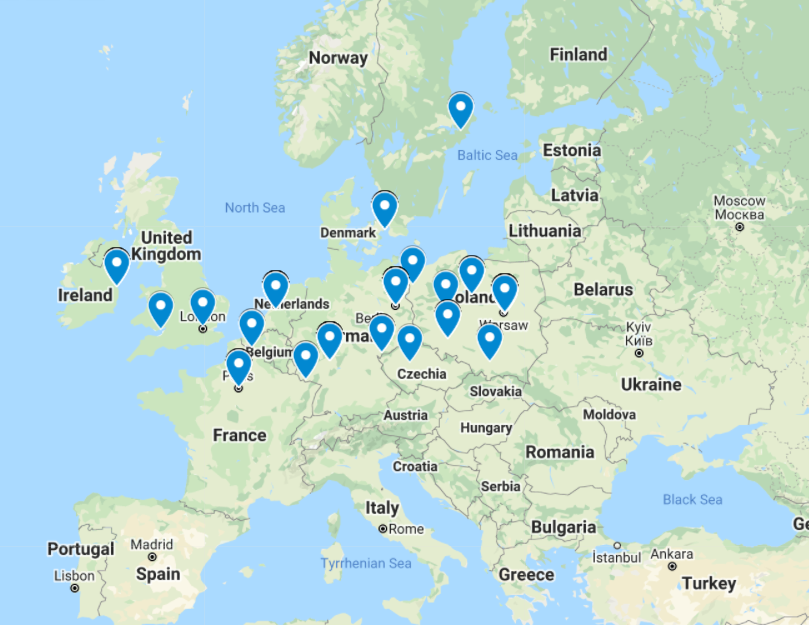
\includegraphics[width=6.5cm]{Wroclavia_map_eu}\\
                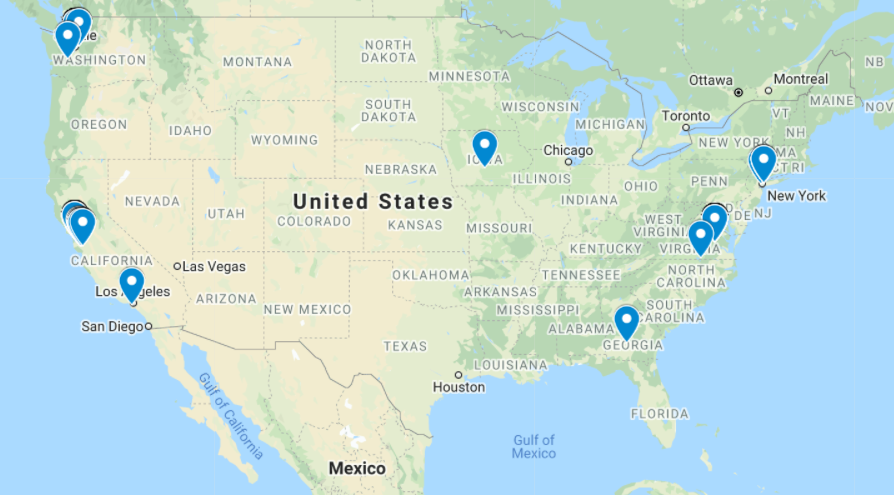
\includegraphics[width=6.5cm]{Wroclavia_map_us}\\
                \textbf{KD Lubin-Wrocław:}\\~\\
                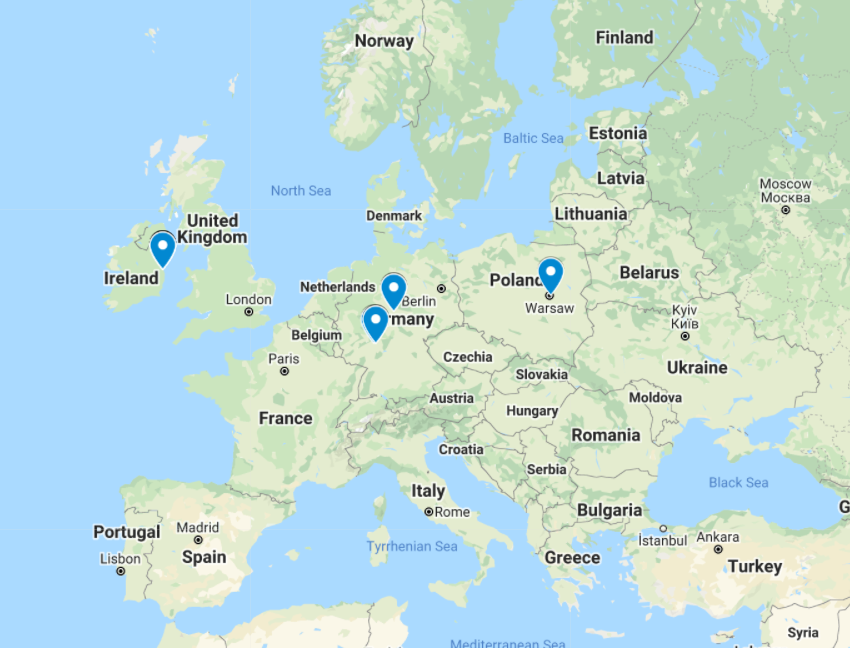
\includegraphics[width=6.5cm]{KD_map_eu}\\
                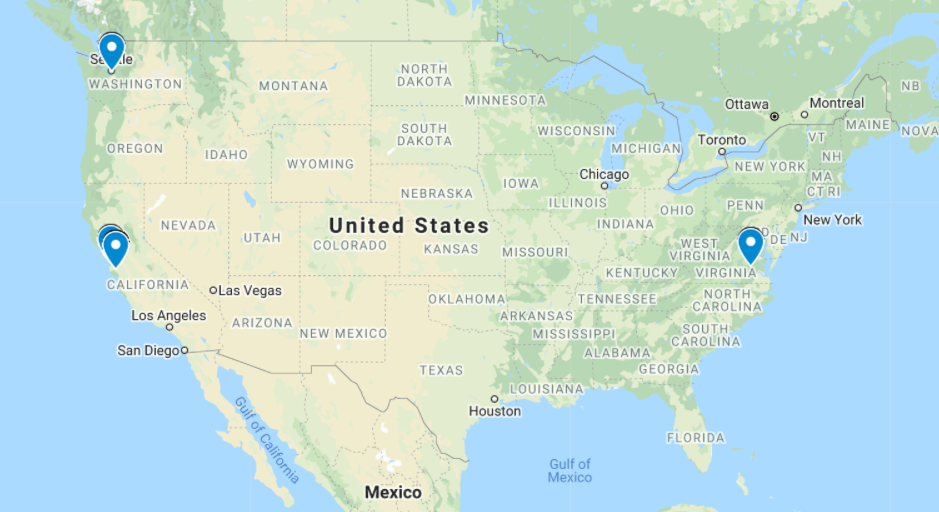
\includegraphics[width=6.5cm]{KD_map_us}\\
            \end{center}
        \end{multicols}
    \section{Wnioski}
        Większość użytkowników smartfonów bądź laptopów w miejscach publicznych w 2021 korzysta z własnego internetu w celu połączenia się z siecią. W odróżnieniu od paru lat wstecz, aktualnie takowy internet pozwala na duży transfer danych przy stosunkowo niskiej cenie. Korzystanie z własnego pakietu internetu jest dodatkowym środkiem bezpieczeństwa gdyż, jak powyższy raport przedstawia, każda sieć otwarta jest podatna na podsłuchiwanie, co może spowodować utratę danych na rzecz niepowołanej osoby.
\end{document}